% Chapter 1

\chapter{Background Concepts} % Main chapter title

\label{Chapter2} % For referencing the chapter elsewhere, use \ref{Chapter1} 

\lhead{Chapter 2. \emph{Background Concepts}} % This is for the header on each page - perhaps a shortened title

%----------------------------------------------------------------------------------------
\section{Neural Networks}

Machine learning research has been growing rapidly over the past decade, with most of this progress coming from deep neural networks (DNNs). These models are powerful tools that can learn to recognize patterns in data, and they have been instrumental in many recent successes in the field.

Neural networks have been studied and developed for many years, with early work on the topic appearing in the late 1950s\cite{Rosenblatt1958ThePA}. One of the most influential papers in this field is the 1986 paper\cite{Rumelhart1986LearningRB}, which introduced the backpropagation algorithm for updating the weights of the network using partial derivatives. This paper and its methods are still used today in modern deep learning.

% This method was successful for shallower networks, but it was very difficult to train deeper networks because of the computational limits at that time. DNNs did not gain much popularity until the early 2010s when the growth of data and increased computational power resulted in a boom in this field.

\subsection{Neurons}

Neural networks were designed to simulate the way the brain learns. This is why they are structured like interconnected neurons passing information, similar to how neurons fire in the human brain. 
A neuron performs the same task as a mathematical function. It takes in a weighted sum of the inputs connected to it, adds a bias term, and passes this sum through a non-linear function also called the activation function. The equation is given below:

\begin{equation}
h = \underbrace{\sum_{i=1}^{\textit{k}} {W_i}{X_i}}_{\mathclap{\text{Weighted Sum of Input Neurons}}} +\smash{\overbrace{b}^{\mathclap{\text{Bias Term}}}}
\end{equation}

\begin{equation}
Y = \underbrace{\huge{\textit{f}}}_{\mathclap{\text{Non-Linear Activation}}} \, \bigl( h \bigr)  = \text{Neuron Output}
\end{equation}




\subsection{Structure}


\begin{figure}[htbp]
  \centering
    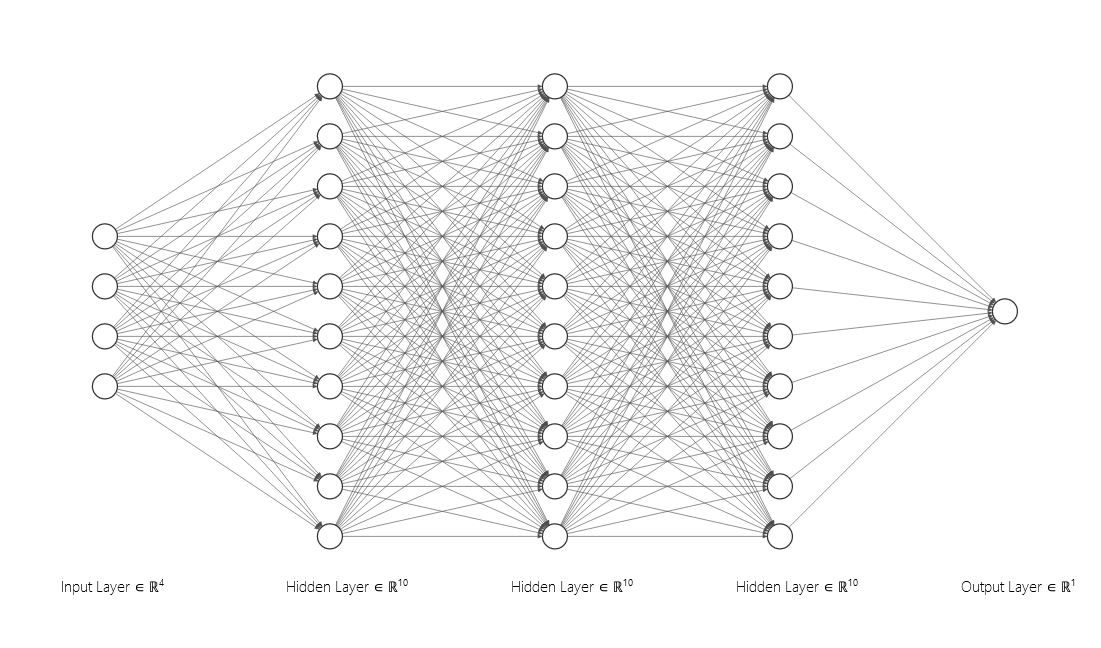
\includegraphics[scale=0.7]{Figures/nn_basic_fig.JPG}
    \rule{35em}{0.5pt}
  \caption[Vanilla Neural Network]{Basic Neural Network}
  \Source{https://alexlenail.me/NN-SVG/}
  \label{fig:basic_nn}
\end{figure}

DNNs consists of mainly three components:
\begin{itemize}[noitemsep,topsep=0pt]
    \item Input Layer
    \item \textit{n} number of Hidden Layers
    \item Output Layer
\end{itemize}

The input layer is the first layer in the network and is responsible for taking in the input. This input is then passed on to the next hidden layer, and so on until the last hidden layer. From the last hidden layer, the information is passed on to the output layer. At the output layer, the model output is used to calculate the loss. The loss is a measure of how far off the prediction of the network is as compared to the actual output. This loss is then backpropagated through the neural network thus updating the model weights.

% Welcome to this \LaTeX{} Thesis Template, a beautiful and easy to use template for writing a thesis using the \LaTeX{} typesetting system.

% If you are writing a thesis (or will be in the future) and its subject is technical or mathematical (though it doesn't have to be), then creating it in \LaTeX{} is highly recommended as a way to make sure you can just get down to the essential writing without having to worry over formatting or wasting time arguing with your word processor.

% \LaTeX{} is easily able to professionally typeset documents that run to hundreds or thousands of pages long. With simple mark-up commands, it automatically sets out the table of contents, margins, page headers and footers and keeps the formatting consistent and beautiful. One of its main strengths is the way it can easily typeset mathematics, even \emph{heavy} mathematics. Even if those equations are the most horribly twisted and most difficult mathematical problems that can only be solved on a super-computer, you can at least count on \LaTeX{} to make them look stunning.

%----------------------------------------------------------------------------------------

